\section{Method} \label{sec:method}
The social network presented here is based on an estimate of the many characters' connections in \got. The table follows Beniwal's approach and dataset \citep{beniwal_network_2018}, but includes positive and negative weights indicating a supportive or averse relationship. "Two characters are considered to co-occur if their names appear in the vicinity of 15 words from one another in the books" \citep{beniwal_network_2018} and characters with fewer than three interactions haven't been included either. The number of occurrences then is denoted as the weight of the tie, which is then rated by a "+" or "-". A "-" has only been used if the characters truly oppose each other, a positive attitude towards each other and a mere coexistence have been labeled as "+". Even if not all "+" relationships support each other fully, low support is also reflected in the number of occurrences. The table is structured as follows:

\begin{table}[h!]
\centering
 \begin{tabular}{llr}
 \toprule
\textbf{Source}	&	\textbf{Target}	&	\textbf{Weight}	\\
\midrule
    Alliser-Thorne	&	Jon-Snow	&	-	32	\\
    Alliser-Thorne	&	Samwell-Tarly	&	-	8	\\
    Arya-Stark	&	Cersei-Lannister	&	-	12	\\
    Arya-Stark	&	Joffrey-Baratheon	&	-	39	\\
    Arya-Stark	&	Petyr-Baelish	&	-	3	\\
    Benjen-Stark	&	Cersei-Lannister	&	-	3	\\
    Aemon-Targaryen-(Maester-Aemon)	&	Jon-Snow	&	+	34	\\
    Aemon-Targaryen-(Maester-Aemon)	&	Samwell-Tarly	&	+	5	\\
    Arya-Stark	&	Benjen-Stark	&	+	3	\\
    Arya-Stark	&	Bran-Stark	&	+	14	\\
    Arya-Stark	&	Catelyn-Stark	&	+	5	\\
    Arya-Stark	&	Eddard-Stark	&	+	30	\\
    Arya-Stark	&	Jon-Snow	&	+	37	\\
    Arya-Stark	&	Rickon-Stark	&	+	7	\\
    Arya-Stark	&	Robb-Stark	&	+	15	\\
    Arya-Stark	&	Sansa-Stark	&	+	104	\\
    ... & ... & ...\\
 \bottomrule
\end{tabular}
\caption{A part of the adjacency list with weights for the characters' connections.}
\label{table:data}
\end{table}

The network graph has been analyzed using \texttt{R} and the \texttt{igraph} package. The package offers the convenience to calculate the most important measures while also enabling complex plots.\\
The graph itself is a complete undirected one-mode network, all actors come from the same dataset.  Relations are modeled as co-occurences and attitudes. Different centrality measures will give estimates about who might be the most important character in the show. The cluster method used is a random walk cluster.

\begin{figure}
    \centering
    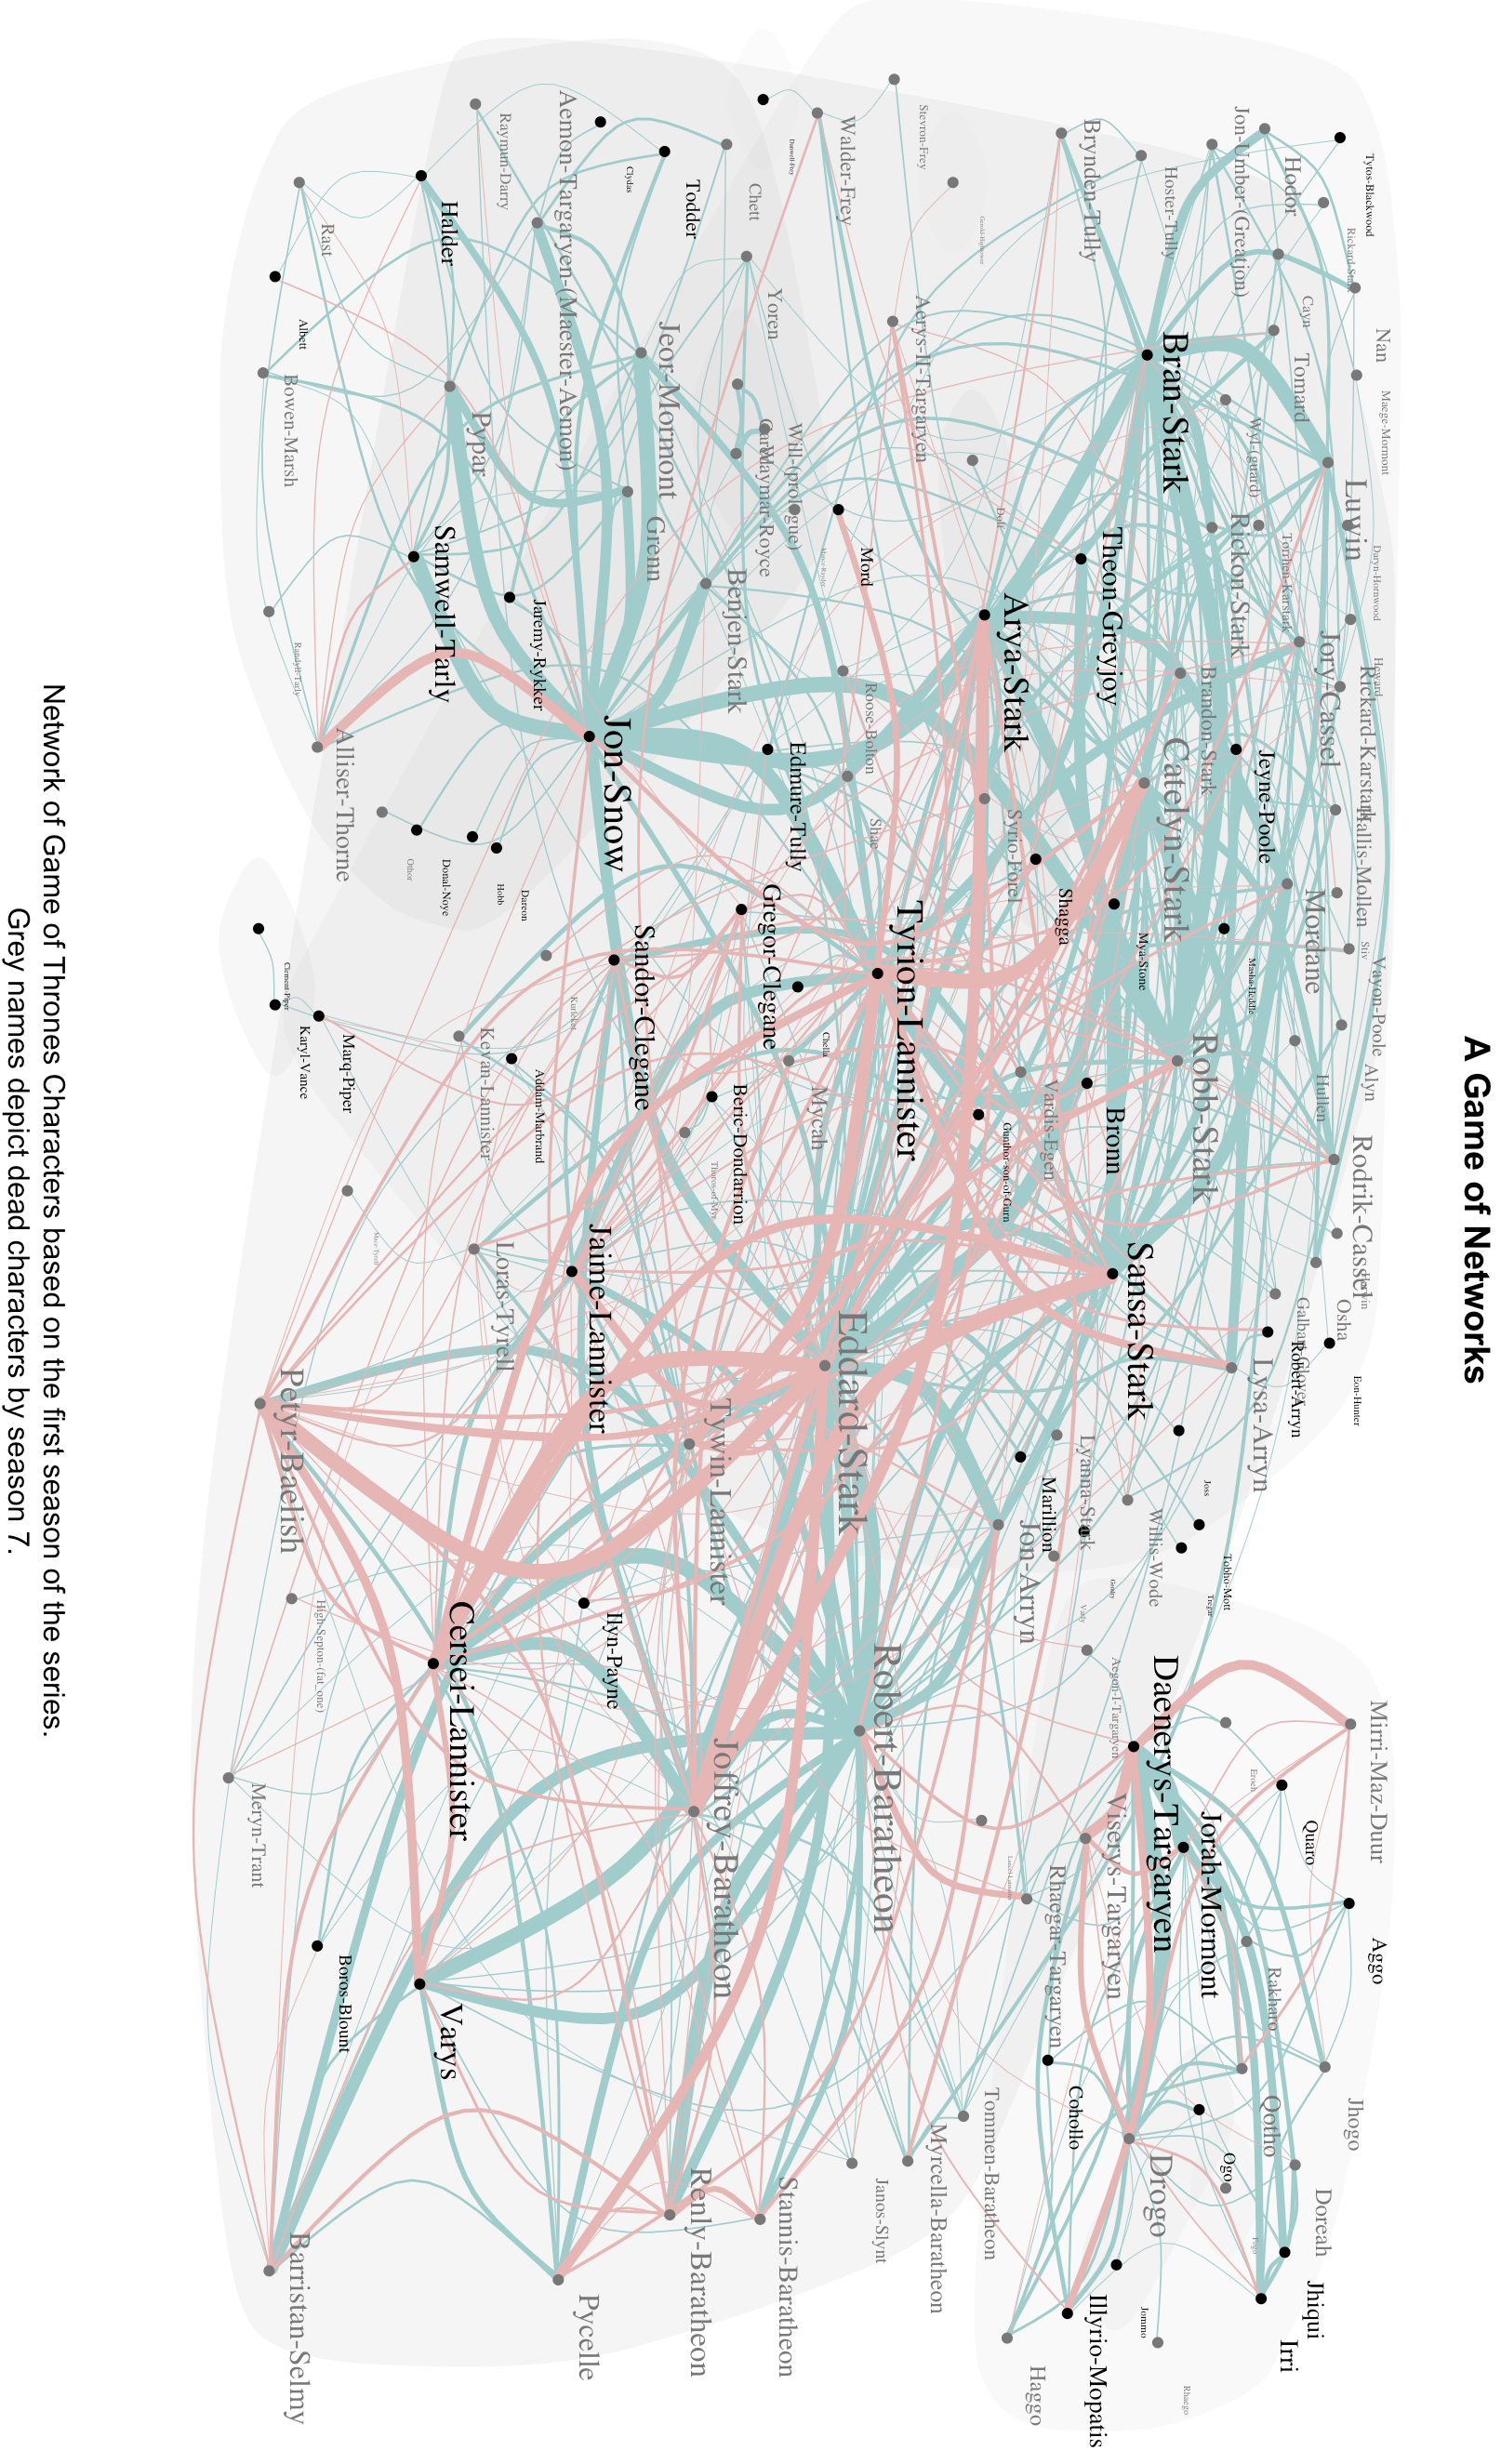
\includegraphics[scale=0.4]{plots/GOTplot.png}
    \caption{The social network of \got.}
    \label{fig:GOTplot}
\end{figure}